
%% bare_conf.tex
%% V1.4b
%% 2015/08/26
%% by Michael Shell
%% See:
%% http://www.michaelshell.org/
%% for current contact information.
%%
%% This is a skeleton file demonstrating the use of IEEEtran.cls
%% (requires IEEEtran.cls version 1.8b or later) with an IEEE
%% conference paper.
%%
%% Support sites:
%% http://www.michaelshell.org/tex/ieeetran/
%% http://www.ctan.org/pkg/ieeetran
%% and
%% http://www.ieee.org/

%%*************************************************************************
%% Legal Notice:
%% This code is offered as-is without any warranty either expressed or
%% implied; without even the implied warranty of MERCHANTABILITY or
%% FITNESS FOR A PARTICULAR PURPOSE! 
%% User assumes all risk.
%% In no event shall the IEEE or any contributor to this code be liable for
%% any damages or losses, including, but not limited to, incidental,
%% consequential, or any other damages, resulting from the use or misuse
%% of any information contained here.
%%
%% All comments are the opinions of their respective authors and are not
%% necessarily endorsed by the IEEE.
%%
%% This work is distributed under the LaTeX Project Public License (LPPL)
%% ( http://www.latex-project.org/ ) version 1.3, and may be freely used,
%% distributed and modified. A copy of the LPPL, version 1.3, is included
%% in the base LaTeX documentation of all distributions of LaTeX released
%% 2003/12/01 or later.
%% Retain all contribution notices and credits.
%% ** Modified files should be clearly indicated as such, including  **
%% ** renaming them and changing author support contact information. **
%%*************************************************************************


% *** Authors should verify (and, if needed, correct) their LaTeX system  ***
% *** with the testflow diagnostic prior to trusting their LaTeX platform ***
% *** with production work. The IEEE's font choices and paper sizes can   ***
% *** trigger bugs that do not appear when using other class files.       ***                          ***
% The testflow support page is at:
% http://www.michaelshell.org/tex/testflow/



\documentclass[conference, ngerman]{IEEEtran}
% Some Computer Society conferences also require the compsoc mode option,
% but others use the standard conference format.
%
% If IEEEtran.cls has not been installed into the LaTeX system files,
% manually specify the path to it like:
% \documentclass[conference]{../sty/IEEEtran}

\usepackage[utf8]{inputenc}
\usepackage[ngerman]{babel}


% Some very useful LaTeX packages include:
% (uncomment the ones you want to load)


% *** MISC UTILITY PACKAGES ***
%
%\usepackage{ifpdf}
% Heiko Oberdiek's ifpdf.sty is very useful if you need conditional
% compilation based on whether the output is pdf or dvi.
% usage:
% \ifpdf
%   % pdf code
% \else
%   % dvi code
% \fi
% The latest version of ifpdf.sty can be obtained from:
% http://www.ctan.org/pkg/ifpdf
% Also, note that IEEEtran.cls V1.7 and later provides a builtin
% \ifCLASSINFOpdf conditional that works the same way.
% When switching from latex to pdflatex and vice-versa, the compiler may
% have to be run twice to clear warning/error messages.






% *** CITATION PACKAGES ***
%
%\usepackage{cite}
% cite.sty was written by Donald Arseneau
% V1.6 and later of IEEEtran pre-defines the format of the cite.sty package
% \cite{} output to follow that of the IEEE. Loading the cite package will
% result in citation numbers being automatically sorted and properly
% "compressed/ranged". e.g., [1], [9], [2], [7], [5], [6] without using
% cite.sty will become [1], [2], [5]--[7], [9] using cite.sty. cite.sty's
% \cite will automatically add leading space, if needed. Use cite.sty's
% noadjust option (cite.sty V3.8 and later) if you want to turn this off
% such as if a citation ever needs to be enclosed in parenthesis.
% cite.sty is already installed on most LaTeX systems. Be sure and use
% version 5.0 (2009-03-20) and later if using hyperref.sty.
% The latest version can be obtained at:
% http://www.ctan.org/pkg/cite
% The documentation is contained in the cite.sty file itself.






% *** GRAPHICS RELATED PACKAGES ***
%
\ifCLASSINFOpdf
  \usepackage[pdftex]{graphicx}
  % declare the path(s) where your graphic files are
  % \graphicspath{{../pdf/}{../jpeg/}}
  % and their extensions so you won't have to specify these with
  % every instance of \includegraphics
  % \DeclareGraphicsExtensions{.pdf,.jpeg,.png}
\else
  % or other class option (dvipsone, dvipdf, if not using dvips). graphicx
  % will default to the driver specified in the system graphics.cfg if no
  % driver is specified.
  \usepackage[dvips]{graphicx}
  % declare the path(s) where your graphic files are
  % \graphicspath{{../eps/}}
  % and their extensions so you won't have to specify these with
  % every instance of \includegraphics
  % \DeclareGraphicsExtensions{.eps}
\fi
% graphicx was written by David Carlisle and Sebastian Rahtz. It is
% required if you want graphics, photos, etc. graphicx.sty is already
% installed on most LaTeX systems. The latest version and documentation
% can be obtained at: 
% http://www.ctan.org/pkg/graphicx
% Another good source of documentation is "Using Imported Graphics in
% LaTeX2e" by Keith Reckdahl which can be found at:
% http://www.ctan.org/pkg/epslatex
%
% latex, and pdflatex in dvi mode, support graphics in encapsulated
% postscript (.eps) format. pdflatex in pdf mode supports graphics
% in .pdf, .jpeg, .png and .mps (metapost) formats. Users should ensure
% that all non-photo figures use a vector format (.eps, .pdf, .mps) and
% not a bitmapped formats (.jpeg, .png). The IEEE frowns on bitmapped formats
% which can result in "jaggedy"/blurry rendering of lines and letters as
% well as large increases in file sizes.
%
% You can find documentation about the pdfTeX application at:
% http://www.tug.org/applications/pdftex





% *** MATH PACKAGES ***
%
%\usepackage{amsmath}
% A popular package from the American Mathematical Society that provides
% many useful and powerful commands for dealing with mathematics.
%
% Note that the amsmath package sets \interdisplaylinepenalty to 10000
% thus preventing page breaks from occurring within multiline equations. Use:
%\interdisplaylinepenalty=2500
% after loading amsmath to restore such page breaks as IEEEtran.cls normally
% does. amsmath.sty is already installed on most LaTeX systems. The latest
% version and documentation can be obtained at:
% http://www.ctan.org/pkg/amsmath





% *** SPECIALIZED LIST PACKAGES ***
%
%\usepackage{algorithmic}
% algorithmic.sty was written by Peter Williams and Rogerio Brito.
% This package provides an algorithmic environment fo describing algorithms.
% You can use the algorithmic environment in-text or within a figure
% environment to provide for a floating algorithm. Do NOT use the algorithm
% floating environment provided by algorithm.sty (by the same authors) or
% algorithm2e.sty (by Christophe Fiorio) as the IEEE does not use dedicated
% algorithm float types and packages that provide these will not provide
% correct IEEE style captions. The latest version and documentation of
% algorithmic.sty can be obtained at:
% http://www.ctan.org/pkg/algorithms
% Also of interest may be the (relatively newer and more customizable)
% algorithmicx.sty package by Szasz Janos:
% http://www.ctan.org/pkg/algorithmicx




% *** ALIGNMENT PACKAGES ***
%
\usepackage{array}
\usepackage[justification=centering, font=small]{caption} 
% Frank Mittelbach's and David Carlisle's array.sty patches and improves
% the standard LaTeX2e array and tabular environments to provide better
% appearance and additional user controls. As the default LaTeX2e table
% generation code is lacking to the point of almost being broken with
% respect to the quality of the end results, all users are strongly
% advised to use an enhanced (at the very least that provided by array.sty)
% set of table tools. array.sty is already installed on most systems. The
% latest version and documentation can be obtained at:
% http://www.ctan.org/pkg/array



% *** SUBFIGURE PACKAGES ***
\ifCLASSOPTIONcompsoc
  \usepackage[caption=false,font=normalsize,labelfont=sf,textfont=sf]{subfig}
\else
  \usepackage[caption=false,font=footnotesize]{subfig}
\fi
% subfig.sty, written by Steven Douglas Cochran, is the modern replacement
% for subfigure.sty, the latter of which is no longer maintained and is
% incompatible with some LaTeX packages including fixltx2e. However,
% subfig.sty requires and automatically loads Axel Sommerfeldt's caption.sty
% which will override IEEEtran.cls' handling of captions and this will result
% in non-IEEE style figure/table captions. To prevent this problem, be sure
% and invoke subfig.sty's "caption=false" package option (available since
% subfig.sty version 1.3, 2005/06/28) as this is will preserve IEEEtran.cls
% handling of captions.
% Note that the Computer Society format requires a larger sans serif font
% than the serif footnote size font used in traditional IEEE formatting
% and thus the need to invoke different subfig.sty package options depending
% on whether compsoc mode has been enabled.
%
% The latest version and documentation of subfig.sty can be obtained at:
% http://www.ctan.org/pkg/subfig




% *** FLOAT PACKAGES ***
%
%\usepackage{fixltx2e}
% fixltx2e, the successor to the earlier fix2col.sty, was written by
% Frank Mittelbach and David Carlisle. This package corrects a few problems
% in the LaTeX2e kernel, the most notable of which is that in current
% LaTeX2e releases, the ordering of single and double column floats is not
% guaranteed to be preserved. Thus, an unpatched LaTeX2e can allow a
% single column figure to be placed prior to an earlier double column
% figure.
% Be aware that LaTeX2e kernels dated 2015 and later have fixltx2e.sty's
% corrections already built into the system in which case a warning will
% be issued if an attempt is made to load fixltx2e.sty as it is no longer
% needed.
% The latest version and documentation can be found at:
% http://www.ctan.org/pkg/fixltx2e


%\usepackage{stfloats}
% stfloats.sty was written by Sigitas Tolusis. This package gives LaTeX2e
% the ability to do double column floats at the bottom of the page as well
% as the top. (e.g., "\begin{figure*}[!b]" is not normally possible in
% LaTeX2e). It also provides a command:
%\fnbelowfloat
% to enable the placement of footnotes below bottom floats (the standard
% LaTeX2e kernel puts them above bottom floats). This is an invasive package
% which rewrites many portions of the LaTeX2e float routines. It may not work
% with other packages that modify the LaTeX2e float routines. The latest
% version and documentation can be obtained at:
% http://www.ctan.org/pkg/stfloats
% Do not use the stfloats baselinefloat ability as the IEEE does not allow
% \baselineskip to stretch. Authors submitting work to the IEEE should note
% that the IEEE rarely uses double column equations and that authors should try
% to avoid such use. Do not be tempted to use the cuted.sty or midfloat.sty
% packages (also by Sigitas Tolusis) as the IEEE does not format its papers in
% such ways.
% Do not attempt to use stfloats with fixltx2e as they are incompatible.
% Instead, use Morten Hogholm'a dblfloatfix which combines the features
% of both fixltx2e and stfloats:
%
% \usepackage{dblfloatfix}
% The latest version can be found at:
% http://www.ctan.org/pkg/dblfloatfix




% *** PDF, URL AND HYPERLINK PACKAGES ***
%
%\usepackage{url}
\usepackage[hidelinks]{hyperref}
% url.sty was written by Donald Arseneau. It provides better support for
% handling and breaking URLs. url.sty is already installed on most LaTeX
% systems. The latest version and documentation can be obtained at:
% http://www.ctan.org/pkg/url
% Basically, \url{my_url_here}.




% *** Do not adjust lengths that control margins, column widths, etc. ***
% *** Do not use packages that alter fonts (such as pslatex).         ***
% There should be no need to do such things with IEEEtran.cls V1.6 and later.
% (Unless specifically asked to do so by the journal or conference you plan
% to submit to, of course. )


\usepackage{gensymb}

% correct bad hyphenation here
\hyphenation{op-tical net-works semi-conduc-tor}


\begin{document}
\title{PTC Vuforia vs. Google Tango}
\author{\IEEEauthorblockN{Patrick Fehling}
\IEEEauthorblockA{Hochschule für Technik und Wirtschaft Berlin, Deutschland\\
E-Mail: p.fehling@student.htw-berlin.de}}


\maketitle

\begin{abstract}
	Vuforia und ähnliche markerbasierte Augmented-Reality-Software dominieren seit einiger Zeit im Bereich der mobilen Geräte (Smartphones \& Tablets). Nun stellt Project Tango von Google eine Alternative dar. In dieser Arbeit sollen zunächst beide Technologien beschrieben und anschließend die wesentlichen Unterschiede und Gemeinsamkeiten ermittelt werden. Schließlich stellt sich heraus, dass Google Tango die überlegenere Technologie ist, dies jedoch nicht sofort bedeutet, dass sie Vuforia schnell vom Markt verdrängt.\\
\end{abstract}

\renewcommand\IEEEkeywordsname{Schlüsselbegriffe}
\begin{IEEEkeywords}
	Augmented Reality; Vuforia; Google Tango; ARToolkit; Microsoft Kinect V2.
\end{IEEEkeywords}

% !TEX root = main.tex

\section{Einleitung}

1968 entwickelte Ivan Sutherland das erste "`Head-Mounted Display"', welches simple Netzstrukturen anzeigen konnte. Dies gilt heute als Grundstein für Virtual (VR) und Augmented Reality (AR). 1992 wurde dann erstmals der Begriff "`augmented reality"' von Tom Caudell und David Mizell geprägt. Seitdem wuchs dieser Forschungsbereich stark an. Mehrere spezialisierte Konferenzen wurden gegründet und verschiedene Technologien wurden entwickelt \cite{ar_history}. Im Wesentlichen funktionieren diese entweder mit markerlosem oder markerbasiertem Tracking.\par
Im Folgenden soll ein Überblick über die Funktionsweise und Möglichkeiten von je einem Stellvertreter gegeben werden. Das ist PTC Vuforia für das markerbasierte Tracking und Google Tango für das markerlose.\par
Daraus wird sich ergeben, dass Google Tango technologisch aufgrund der größeren Datenmenge besser ist. Da Vuforia aber auf allen aktuellen mobilen Geräten mit einer Kamera funktioniert, hat es große Chancen auch weiterhin zu bestehen.
% !TEX root = main.tex

\section{Vuforia}

Vuforia ist ein auf Markern basierendes Software Development Kit für Augmented Reality, welches von Qualcomm entwickelt und später von PTC gekauft wurde. Die Marker werden über Bilderkennungsalgorithmen erkannt, d.h. für den Einsatz ist lediglich ein Computer und eine Kamera notwendig. Somit kann das SDK auf einer Reihe von Geräten und Plattformen eingesetzt werden, dazu zählen: Android- und iOS-Smartphones und -Tablets, Notebooks und auch AR-Brillen wie die Microsoft HoloLens \cite{vuforia_devices}. Das SDK ist jedoch proprietär. Aus diesem Grund kann die Funktionsweise hier nur rekonstruiert werden.

\subsection{Marker}
Marker können theoretisch beliebige Bilder oder auch dreidimensionale Objekte sein. Jedoch müssen diese bestimmte Merkmale besitzen, um das Tracking zu ermöglichen. Diese Merkmale heißen Features und je mehr davon vorhanden sind, desto besser ist das vom Vuforia Developer Portal vergebene Rating. Kein Stern bedeutet hier, dass der Marker nicht zum Tracken geeignet ist und fünf Sterne stellen das Optimum dar. Ersteres wäre ein Bild, welches nur Rundungen und weiche Farbübergange und wenig Kontrast bietet. Ein Beispiel für einen optimalen Marker ist in Abbildung \ref{vuforia_stones_image} zu sehen. Das untere Bild in der Abbildung zeigt die Features des Bildes. "`A feature is a sharp, spiked, chiseled detail in the image, [...]."'\cite{features} Viele eckige oder kantige Details in einem Bild sorgen also für viele Features. Eine Erhöhung des Kontrastes führt meist zu einer Verbesserung des Ratings. Darüber hinaus sollten jedoch sich wiederholende Muster von Features in einem Bild vermieden und auf eine gleichmäßige Verteilung geachtet werden, da sonst für das Tracking mehr vom Bild zu sehen sein müsste.

\begin{figure}[h]
	\centering
	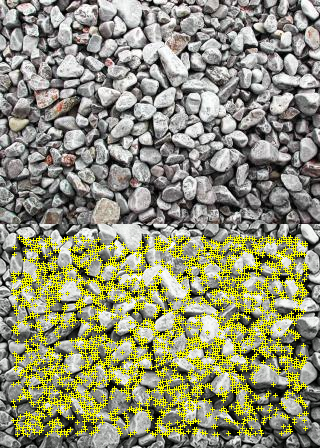
\includegraphics[width=2.5in]{pictures/vuforia_stones_comparison}
	\caption{Vuforia-Steine: Optimal trackbares Markerbild\newline (Quelle: Vuforia Developer Portal)}
	\label{vuforia_stones_image}
\end{figure}

\subsection{"`Hello-World"'-Anwendung}
Im Rahmen dieser Seminararbeit wurde eine "`Hello World"'-Anwendung für Android entwickelt, um ein Gefühl von der Funktionsweise des SDKs zu bekommen. Diese kann in Abbildung \ref{vuforia_sample} betrachtet werden. Hierbei wurde der in Abbildung \ref{vuforia_stones_image} zu sehende Marker verwendet. Sobald dieser von der Anwendung erfasst wird, werden die AR-Elemente projiziert. Wenn das Handy bewegt wird, bleibt der Roboter an der gleichen Stelle stehen. Wenn man den Marker bewegt, bewegt sich der Roboter mit diesem.\par
Für das initiale Erkennen des Markers ist aufgefallen, dass dieser zum Großteil von der Kamera erfasst sein muss. Anschließend kann sich jedoch ein Großteil auch außerhalb des Sichtfelds der Kamera befinden. Dies hat wahrscheinlich mit der hohen Feature-Anzahl des Bildes zu tun. Vermutlich dienen Gruppen von Features als Schlüssel zum Erkennen des Markers. Ein zweiter Marker mit weniger Features wird schwerer erkannt und darauf projizierte Objekte verschwinden schneller, sobald Teile des Markers verdeckt oder sich außerhalb des Bildes befinden.

\begin{figure}[h]
	\centering
	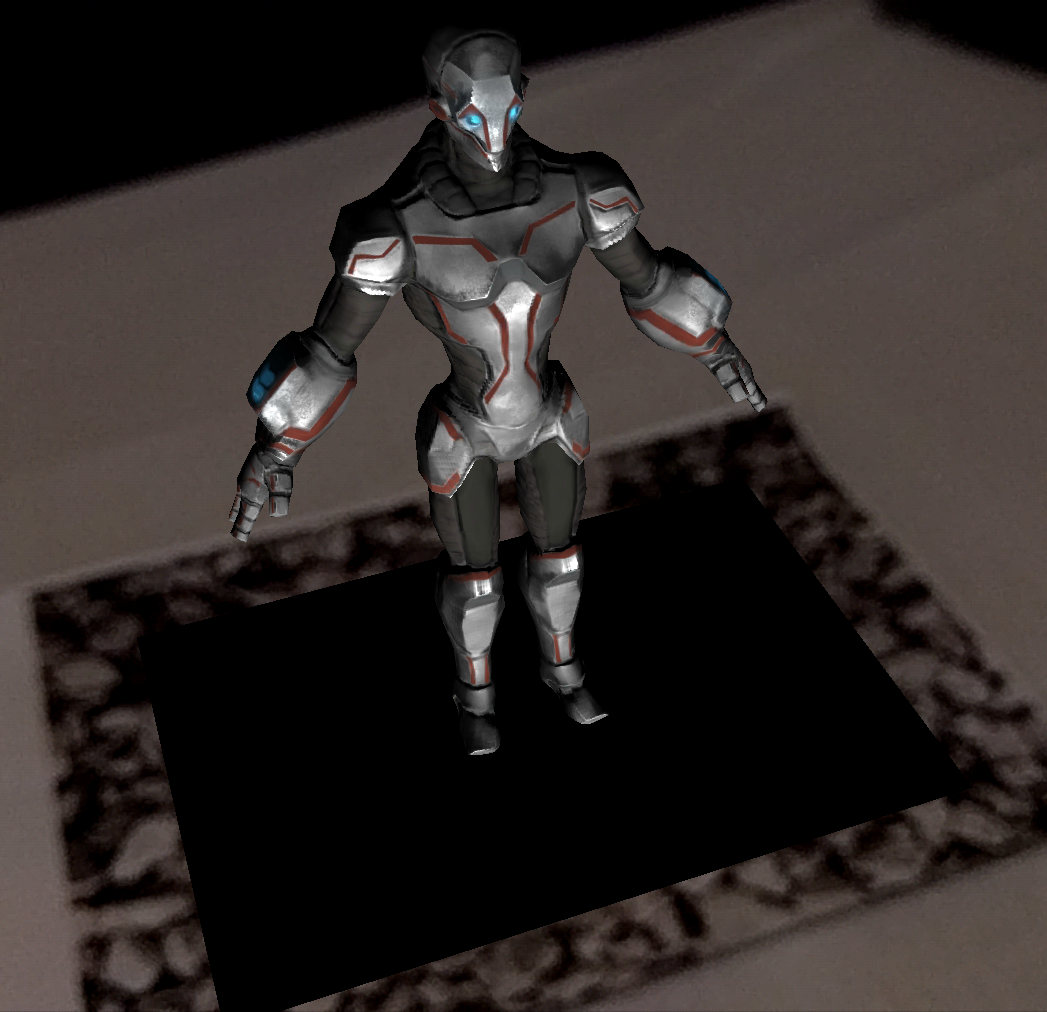
\includegraphics[width=2.5in]{pictures/vuforia_sample2}
	\caption{Auf dem Marker werden die AR-Elemente projiziert.\newline (Quelle: Autor)}
	\label{vuforia_sample}
\end{figure}

\subsection{ARToolKit}
Wenn man diese Schlüssel einzeln betrachtet, liegt der Vergleich mit dem ARToolKit \cite{artoolkit1}\cite{artoolkit2} nahe. Dabei werden ebenfalls Marker verwendet. Dort werden diese jedoch mit einem schwarzen Rahmen hervorgehoben und sollten nur einfache schwarze Muster enthalten. Das Bild der Kamera wird nach diesem Marker abgetastet. Sobald ein Marker gefunden wurde, wird seine Orientierung und Position anhand des gespeicherten Markers ermittelt. 3D-Objekte werden dann so projiziert, dass sie genauso ausgerichtet sind wie der Marker.\par
Nachteile sind hierbei, dass die Marker sehr simpel gehalten werden und immer vollständig sichtbar sein müssen. Ein sehr effizientes Beispiel hierfür ist zum Beispiel eine 3x3-Matrix, wobei jedes Feld entweder weiß oder schwarz ist. Daraus können sich dann mehrere Marker ableiten, die auch zusammen in einer Anwendung benutzt werden können. Hierbei ist noch zu beachten, dass jeder Marker einzigartig sein muss auch wenn er gedreht wird, d.h. ein weißes Feld in der oberen rechten Ecke der Matrix erzeugt den gleichen Marker wie ein weißes Feld in der unteren rechten Ecke, sofern der Rest schwarz ist.\par
Da Marker bei Vuforia nicht immer vollständig sichtbar sein müssen, scheint ein Marker also nicht nur \textbf{ein} Marker zu sein sondern besteht aus vielen einzelnen, welche sich aus den Features ergeben.

\subsection{Beispielanwendung}
Eine Android-App wurde an der Takming University of Science and Technology in Taipei zur Verbesserung des Lernens entwickelt\cite{vuforia_sample_application}. Diese wurde für diese Arbeit ausgewählt, da diese am besten dokumentiert ist und auch mehr Hintergründe von der Anwendung und Vuforia zeigt. Andere Apps, welche man z.B. über die Vufora-Webseite findet sind meist proprietär. Dazu zählen bspw. eine App von BMW, womit man ein Auto in seine Einfahrt projizieren kann und eine ähnliche App von Samsung für Fernseher im Wohnzimmer.\par
Bei dieser Applikation wurden Meereslebewesen auf die Marker projiziert, um diese besser analysieren zu können. Über ebenfalls projizierte Buttons können die Grafiken gewechselt werden. Das Aussehen und die Bewegungsmuster der Lebewesen soll den Studierenden so besser vermittelt werden können. Zusätzliche Informationen werden über eine Textbox unter der Figur dargestellt.

% !TEX root = main.tex

\section{Google Tango}

Google Tango ist ein Projekt, welches markerlose Augmented-Reality-Applikationen über mehrere Kameras und Tiefensensoren ermöglicht. Bisher sind drei Geräte veröffentlicht worden, welche diese Technologie besitzen. Das erste und zweite Development Kit und das zum Zeitpunkt dieser Seminararbeit bald erscheinende Smartphone von Lenovo. Im folgenden wird hauptsächlich das zweite Development Kit behandelt. Dies ist ein Tablet mit einem 7 Zoll großen Full-HD-Touchscreen-Display, einer 4 MP RGB-IR Kamera kombiniert mit einer 170\degree\/ Kamera mit Bewegungserkennung \cite{tango_teardown}.\par
Der Aufbau und die Wahl der Kameras erinnert stark an die Kinect V2 der Xbox One von Microsoft, sodass die Funktionalität hier sehr ähnlich sein sollte. Der eingebaute Infrarot-Projektor leuchtet den Raum mit einer Vielzahl unsichtbarer Punkte aus. Diese sind unregelmäßig angeordnet, sodass einzigartige Muster entstehen.\par
Die einzige Einschränkung für dieses Verfahren stellen fremde Infrarot-Quellen dar. So ist dies aufgrund der natürlichen Infrarotstrahlung der Sonne nicht bei Tageslicht möglich und mehrere Geräte würden sich untereinander ebenfalls stören. Völlige Dunkelheit stellt jedoch hierfür kein Problem dar.

\subsection{Tiefenmessung und Tracking}
Bevor eine Tiefenmessung oder ein Tracking von Objekten stattfinden kann, muss das Gerät seine eigene Position so genau wie möglich kennen. Dazu wird zum einen die Motion-Tracking-Kamera verwendet. Durch effiziente Analyse z.B. Kanten und Ecken, nimmt diese Bewegung war und kann damit auch feststellen ob sich das Gerät bewegt. Das allein ist jedoch nicht sehr präzise, da sich auch andere Objekte bewegen können. Durch zusätzliche Informationen vom Gyroskop und dem Beschleunigungssensor, welche in vielen Smartphones verbaut sind, kann die genaue Position des Geräts im Raum ermittelt werden \cite{tango_technology}.\par
Um nun die Tiefe von Objekten zu ermitteln kommen drei Systeme zum Einsatz \cite{kinect_imaging}\cite{depth_perception}:
\subsubsection{Structured Light}
Hierbei wird über die Infrarot-Kamera ein Punktmuster ausgesendet. Der Infrarotsensor nimmt dieses und vergleicht es mit seinem virtuellem Abbild. Je größer ein Punkt erscheint, desto weiter ist er entfernt. Dieses Punktmuster ist in Abbildung \ref{tango_ir_projection} zu sehen.
\subsubsection{Time-of-flight}
Es wird ein Infrarot-Strahl ausgesendet. Dieser wird von einem Objekt reflektiert und vom Infrarotsensor aufgenommen. Die Zeit zwischen dem Senden und Empfangen wird dabei gemessen. Je mehr Zeit der Strahl benötigt desto weiter ist der Punkt von dem der Strahl reflektiert wurde entfernt.
\subsubsection{Stereo-Kameras}
Die Szene wird von zwei Kameras aufgenommen. Durch den bekannten Abstand der Kamera und den Kamerawinkeln zum jeweiligen Punkt kann die Tiefe berechnet werden und so eine Tiefenkarte zur aufgenommen Szene erstellt werden.

\begin{figure}[h]
	\centering
	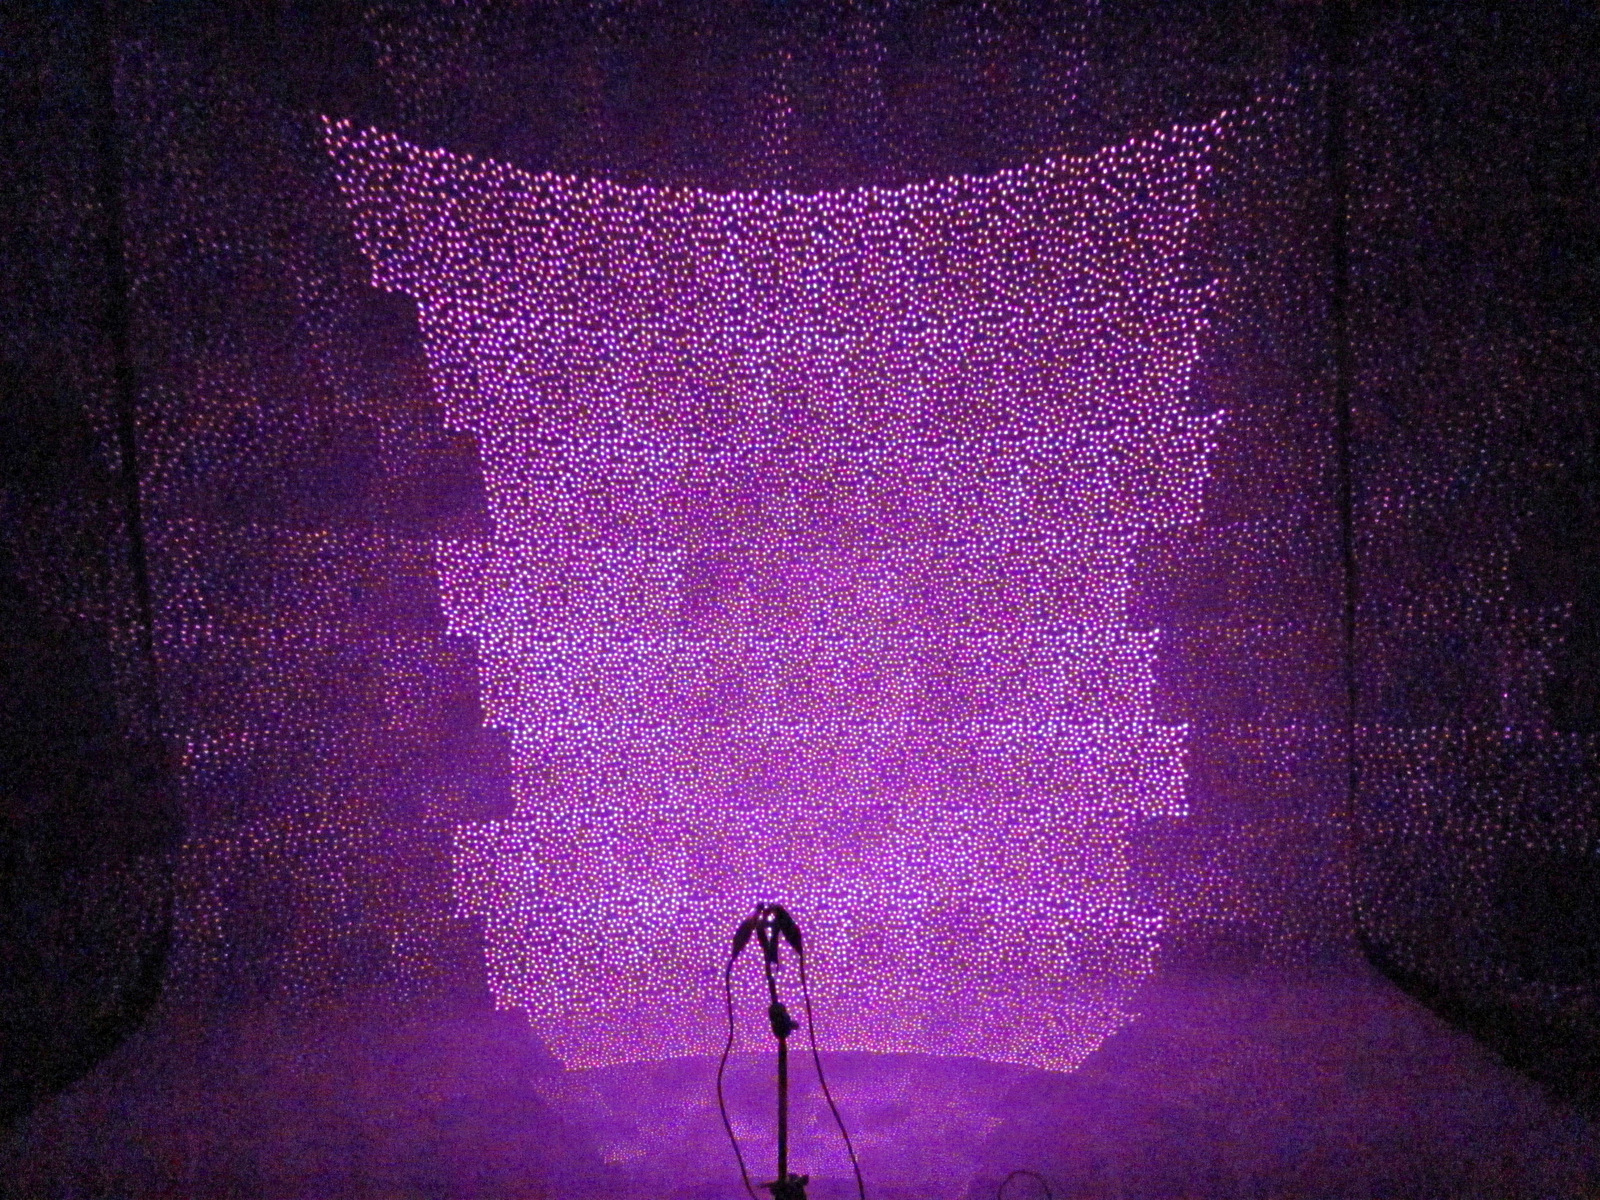
\includegraphics[width=3in]{pictures/tango_ir_projection}
	\caption{Die Umgebung wird mit einem unregelmäßigen Punktmuster per IR-Projektion bestrahlt. (Quelle: \cite{tango_teardown})}
	\label{tango_ir_projection}
\end{figure}

Google Tango liefert die Rohdaten der Technologie als eine sog. "`TangoPointCloud"', welche dann von der eigenen Anwendung verwendet werden kann. Dahinter verbirgt sich im Wesentlichen nichts anderes als ein Array mit allen erfassten Punkten in Form von Koordinaten. Leider ist es mir im Rahmen dieser Arbeit nicht möglich diese Daten selber zu erstellen, da mir die notwendige Hardware zu diesem Zeitpunkt noch nicht zur Verfügung steht.

\subsection{Area Learning \cite{tango_area_learning}}
Diese Rohdaten werden jedoch nicht nur ausgegeben. Sie können durch das Tango Development Kit auch schon verarbeitet werden, um ein "`Gedächtnis"' aufzubauen. Dies nennt sich "`Area Learning"'. Dadurch kann erkannt werden, wann sich das Gerät in einem bekannten Gebiet befindet.\par
Schlüsselelemente der Szene wie Kanten und Ecken werden in einem lokalen Index, dem Area Description File (ADF) gespeichert, um auf diese später wieder zugreifen zu können. Zukünftige Szenen werden dann mit diesen Daten abgeglichen und so kann ungefähr bestimmt werden, wo sich das Gerät bzw. der Nutzer mit dem Gerät befindet. Durch zusätzliche Lokalisierungstechnologien z.B. über WLAN kann das Ergebnis deutlich verbessert werden. Andernfalls können identische Räume, Veränderungen im Raum oder verschiedene Tageszeiten Probleme verursachen. Für letzteres bietet es sich auch an mehrere ADFs zu verwenden, also z.B. eine für die Nacht und eine für den Tag.\par
Des Weiteren soll das Area Learning Fehler des Motion Trackings ausgleichen. Die Position und Ausrichtung des Geräts weicht mit steigender Nutzung von der Position und Ausrichtung, die das Gerät annimmt zu haben, ab. Wenn ein bekanntes Gebiet gefunden wurde, kann dieser Fehler korrigiert werden.

\subsection{Beispielanwendungen \cite{tango_apps}}

\subsubsection{Project Tango Constructor}
Durch diese Anwendung kann die Umgebung mit dem Google Tango-Gerät aufgenommen werden, um daraus ein 3D-Modell zu generieren. Hierbei sind gute Lichtverhältnisse notwendig, sodass die Oberflächen gut abgebildet werden können.

\subsubsection{Project Tango MeasureIt}
Mit dieser Applikation können Strecken auf 2-5\% Genauigkeit \cite{tango_apps} gemessen werden. Für präzise Messungen ist dies ungeeignet, jedoch für die Planung einer Einrichtung o.ä. sollte diese Genauigkeit ausreichend sein. So kann man z.B. einen Türrahmen ausmessen. Solche eine Anwendung der App ist in Abbildung \ref{measure_it} zu sehen
\begin{figure}[h]
	\centering
	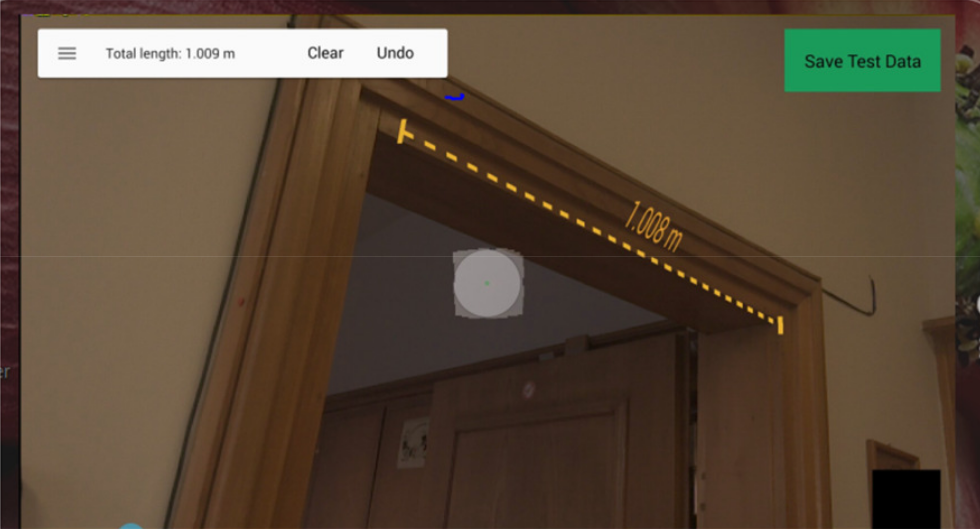
\includegraphics[width=3.25in]{pictures/tango_measure_it}
	\caption{Google Tango App MeasureIt\newline (Quelle: \cite{tango_apps})}
	\label{measure_it}
\end{figure}
% !TEX root = main.tex

\section{Vergleich}
In diesem Abschnitt werden die wesentlichen Punkte beider Technologien zusammengefasst und gegenübergestellt. Besonders hervorzuheben ist, dass die scheinbar größte Schwäche von Vuforia, der Marker, gleichzeitig auch eine Stärke sein kann. Der Marker stellt sicher, dass die Projektion an der richtigen Stelle bleibt. Bei Google Tango müssen dafür zusätzliche Maßnahmen entwickelt werden, z.B. ein Algorithmus zur Berechnung der optimalen Stelle in der PointCloud oder man lässt den Nutzer über UI-Elemente entscheiden. Dies ist natürlich sehr stark vom Verwendungszweck abhängig und gibt dem Entwickler auch eine gewisse Freiheit.\par
Beide haben aber auch mit ähnlichen Problemen zu kämpfen. Dazu gehört bspw. die Reichweite. Ein Marker wird mit zunehmender Entfernung mit immer weniger Pixeln von der Kamera erfasst. Irgendwann kann er dann nicht mehr wahrgenommen werden. Gleiches gilt für die IR-Projektion von Google Tango auch diese hat seine Grenze schnell erreicht.

\begin{table}[h]
	\centering
	\begin{tabular}{|p{4cm}|p{4cm}|}
		\hline
		\textbf{Vuforia} & \textbf{Google Tango}\\
		\hline
		\begin{itemize}
			\setlength\itemsep{0.5em}
			\raggedright
			\item Markerbasiertes Tracking\newline
			$\rightarrow$ Verbindungspunkt zwischen realer und virtueller Welt
			\item benötigt eine Kamera\newline 
			$\rightarrow$ günstiger, aber wenige Inputdaten\newline
			\item verfügbar für viele Geräte und Betriebssysteme
			\item mittlere bis gute Licht-verhältnisse notwendig (Der Marker muss sichtbar sein)
			\item keine Probleme bei Sonnenlicht\newline
			\item nicht lernfähig
		\end{itemize}
		 & 
		 \begin{itemize}
		 	\setlength\itemsep{0.5em}
		 	\raggedright
		 	\item Markerloses Tracking\newline
		 	$\rightarrow$ Viele Möglichkeiten, Projektion jedoch nicht immer trivial
		 	\item benötigt zwei Kameras und einen IR-Projektor $\rightarrow$ teurer, aber viele Inputdaten (z.B. Tiefe)
		 	\item (noch) verfügbar für ein Endverbraucher-Produkt
		 	\item theoretisch auch im Dunkeln verwendbar (abhängig von der Anwendung) \newline
		 	\item starke Beeinträchtigung durch Sonnenlicht oder andere IR-Quellen
		 	\item Lernfähigkeit, "`Gedächtnis"'
		 \end{itemize}\\
		\hline
	\end{tabular}
\end{table}
% !TEX root = main.tex

\section{Fazit}
Wenn wir die beiden Technologien vergleichen ist es schwer zu beurteilen welche besser ist, beide haben ihre Vor- und Nachteile und Einsatzgebiete. Wenn man einen realen Raum in die Virtualität überführen möchte, ist Google Tango durch seine Umgebungswahrnehmung klar im Vorteil. Mit Vuforia hat man jedoch einen physischen Punkt an dem sich reale und virtuelle Welt treffen. Dieser kann vom Nutzer angefasst werden und könnte so entstehende Hürden bei der Nutzung verringern. Sofern der Nutzer z.B. für ein Spiel etwas greifen muss, ist diese Bindung an die reale Welt durchaus von Vorteil. Andererseits ist eine Vuforia-Anwendung ohne Marker in der Regel nutzlos.\par
Die weite Verbreitung von Vuforia ist jedoch nicht nur dem geschuldet, dass es markerlose Technologien für mobile Geräte noch nicht gab. Die Kosteneffizienz ist ebenfalls ein großer Faktor. Es braucht nicht einmal ein Highend-Smartphone, um eine Vuforia-App nutzen zu können. Außerdem gibt es Google Tango nur für Android und das wird sich vermutlich auch nicht so schnell ändern. Aus diesem Gründen könnte sich Tango nur langsam in der Verbreitung durchsetzen.\par
Auf der anderen Seite ist Android ebenfalls von Google, welches auf vielen verschieden Smartphones und Tablets läuft. Es ist also denkbar, dass z.B. in einer zukünftigen Generation der Pixel-Serie die Tango-Technologie verwendet wird und andere Hersteller dann dadurch nachziehen. Ohne diese Unterstützung wird sich diese Technologie wahrscheinlich nur schleichend durchsetzen.\par
Des Weiteren gab es schon lange keine neuen Technologien, die den Einsatzbereich für Smartphones und Tablets merklich erweitern. Der jüngste Vergleich hierzu wäre "`NFC"', welche viele Jahre vom Standard bis zur Integration in einer Vielzahl von Geräten benötigte \cite{nfc_iso}\cite{android_pay}.\par
Alles in allem ist Google Tango jedoch als mächtiger einzuschätzen, da einfach viel mehr Daten zur Verarbeitung zur Verfügung stehen. Man könnte viele Vuforia-Applikationen mit Tango wahrscheinlich nachbilden, indem man dem Raum nach einem Objekt/Marker scannt oder ihn sogar vollständig weglässt und stattdessen dahin projiziert, wo es sich am besten anbietet. Mit Vuforia einen Raum zu scannen oder Tiefe wahrzunehmen ist jedoch völlig unmöglich.

\pagestyle{plain}
\bibliographystyle{plain}
\bibliography{bibliography}

\end{document}


